\begin{figure*}[!ht]
  \centering
  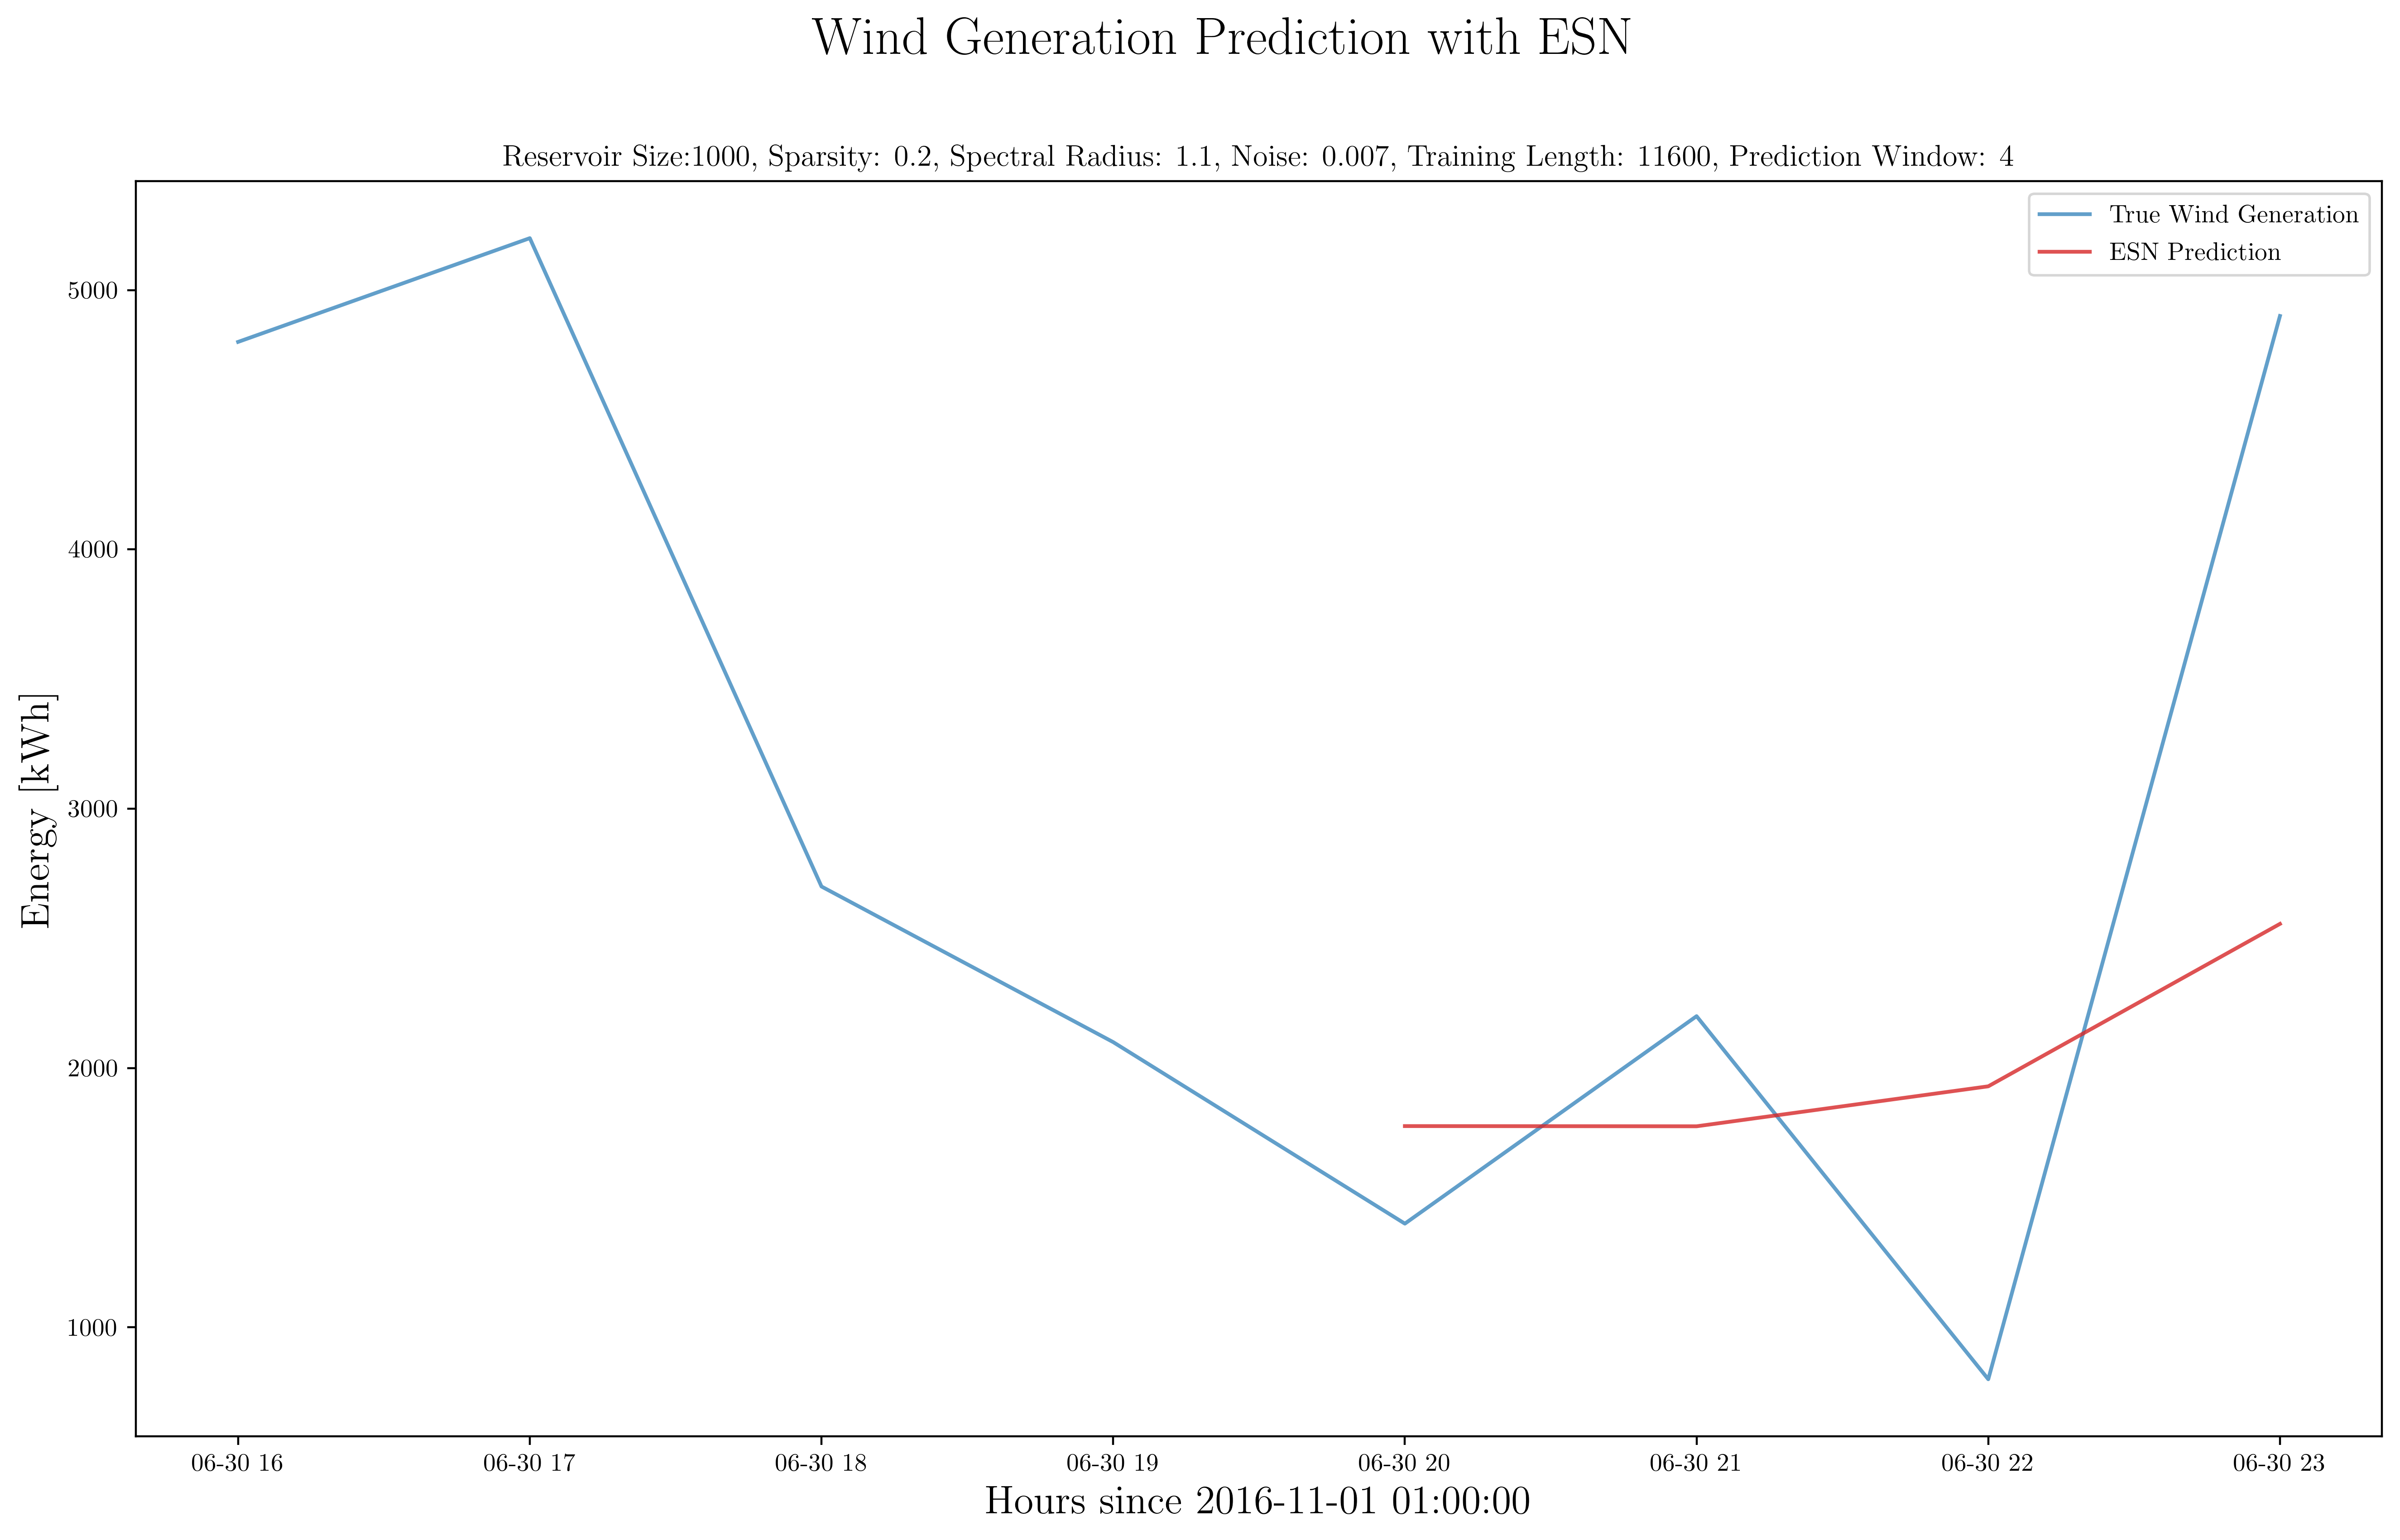
\includegraphics[width=0.8\textwidth]{04_wind_wettemp_prediction.png}
  \caption{The optimized 4 hour ahead wind energy prediction with wet bulb
  temperature as a meteorological predictor.}
  \label{fig:wind04}
\end{figure*}
% \begin{center}
  \begin{table*}[!ht]
    \centering
    \caption{Tabulated error for 4-hour ahead wind forecasts with various coupled quantities. Improvement indicates the percentage improvement over the base case of forecasting wind energy alone.}
    \label{tab:wind04}
    \begin{tabular}{l|c|c|c|c}
      &  & & Improvement & Improvement \\
      Scenario  & MAE & RMSE & MAE (\%) & RMSE (\%)\\
      \hline
      Wind Energy & 0.090266 & 0.124303 & [-] & [-] \\
      Wind + Sun Elevation & 0.039248 & 0.083134 & -56.52& -33.12\\
      Wind + Humidity & 0.064131 & 0.096310 & -28.95& -22.52\\
      Wind + Pressure & 0.043739 & 0.087981 & -51.54& -29.22\\
      Wind + Wet Bulb Temp. & 0.044447 & 0.077770 & -50.76& -37.44\\
      Wind + Dry Bulb Temp. & 0.050536 & 0.083151 & -44.01 & -33.11\\
      Wind + Wind Speed & 0.063456 & 0.088157 & -29.70 & -29.07\\
    \end{tabular}
  \end{table*}
% \end{center}
